\documentclass{standalone}
\usepackage[x11names]{xcolor}
\usepackage{tikz}

\begin{document}

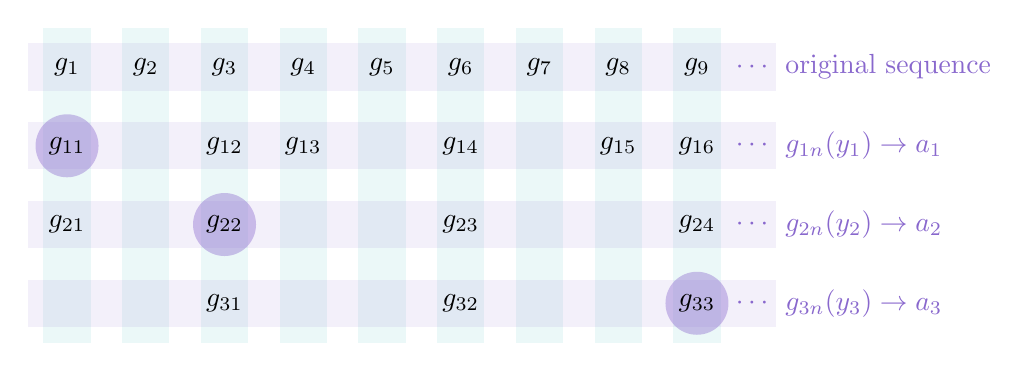
\begin{tikzpicture}
    \fill [MediumPurple3, opacity = 0.1] (0.5, 0.3) rectangle (10, -0.3);
    \node [MediumPurple3] at (9.7, 0) {$\cdots$};
    \node [MediumPurple3, anchor = west] at (10, 0) {original sequence};
    \foreach \i in {1, ..., 9} {
        \fill [DarkSlateGray3, opacity = 0.15] (\i - 0.3, 0.5) rectangle (\i + 0.3, -3.5);
        \node at (\i, 0) {$g_{\i}$};
    }
    \foreach \i\j in {1/1, 3/2, 9/3} {
        \fill [MediumPurple3, opacity = 0.4] (\i, -\j) circle (0.4);
    }

    \foreach \row [count = \m] in {{1, 3, 4, 6, 8, 9}, {1, 3, 6, 9}, {3, 6, 9}} {
        \fill [MediumPurple3, opacity = 0.1] (0.5, -\m + 0.3) rectangle (10, -\m - 0.3);
        \node [MediumPurple3] at (9.7, -\m) {$\cdots$};
        \foreach \i [count = \n] in \row {
            \node at (\i, -\m) {$g_{\m\n}$};
        }
        \node [MediumPurple3, anchor = west] at (10, -\m) {$g_{{\m}n}(y_\m) \to a_{\m}$};
    }            
\end{tikzpicture}

\end{document}